\begin{frame}{Invariant Local Features}
\begin{figure}
    \centering
    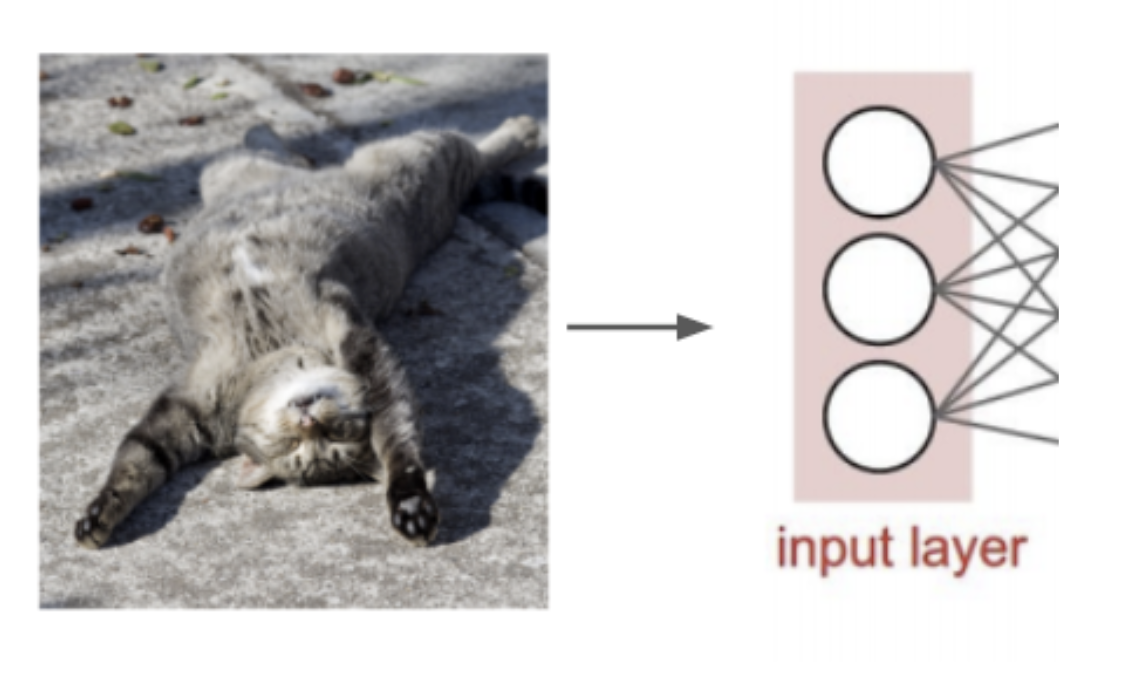
\includegraphics[width=0.9\textwidth]{img/catinput.png}
    \caption{What is the best way to pass an image into a neural network?}
\end{figure}
\end{frame}

\begin{frame}{Invariant Local Features}
\begin{figure}
    \centering
    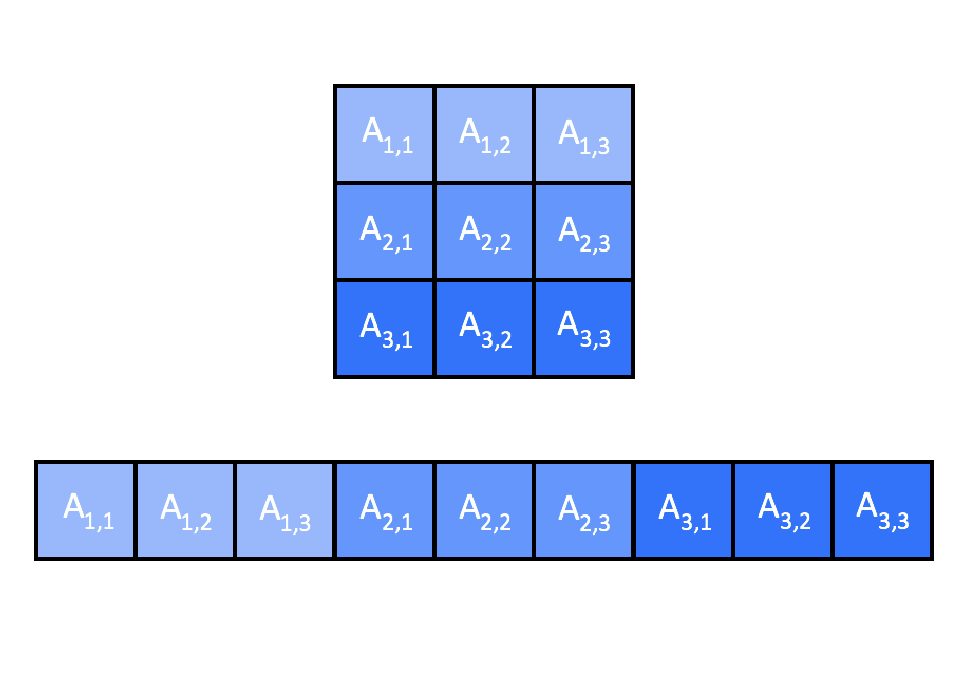
\includegraphics[width=0.7\textwidth]{img/flatten.png}
    \caption{What could be wrong with just flattening images?}
\end{figure}
\end{frame}

\begin{frame}{Invariant Local Features}
What could be wrong with just flattening images?
\begin{itemize}
    \item Images are huge: How many features in a 128x128x3 image?
\end{itemize}
\end{frame}

\begin{frame}{Invariant Local Features}
What could be wrong with just flattening images?
\begin{itemize}
    \item Images are huge: How many features in a 128x128x3 image?
    \item For every change in viewpoint, you would change 49,152 features.
\end{itemize}
\end{frame}

\begin{frame}{Invariant Local Features}
What could be wrong with just flattening images?
\begin{itemize}
    \item Images are huge: How many features in a 128x128x3 image?
    \item For every change in viewpoint, you would change 49,152 features.
    \item You don't take advantage of \textbf{locality}
\end{itemize}
\end{frame}

\begin{frame}{Invariant Local Features}
\begin{figure}
    \centering
    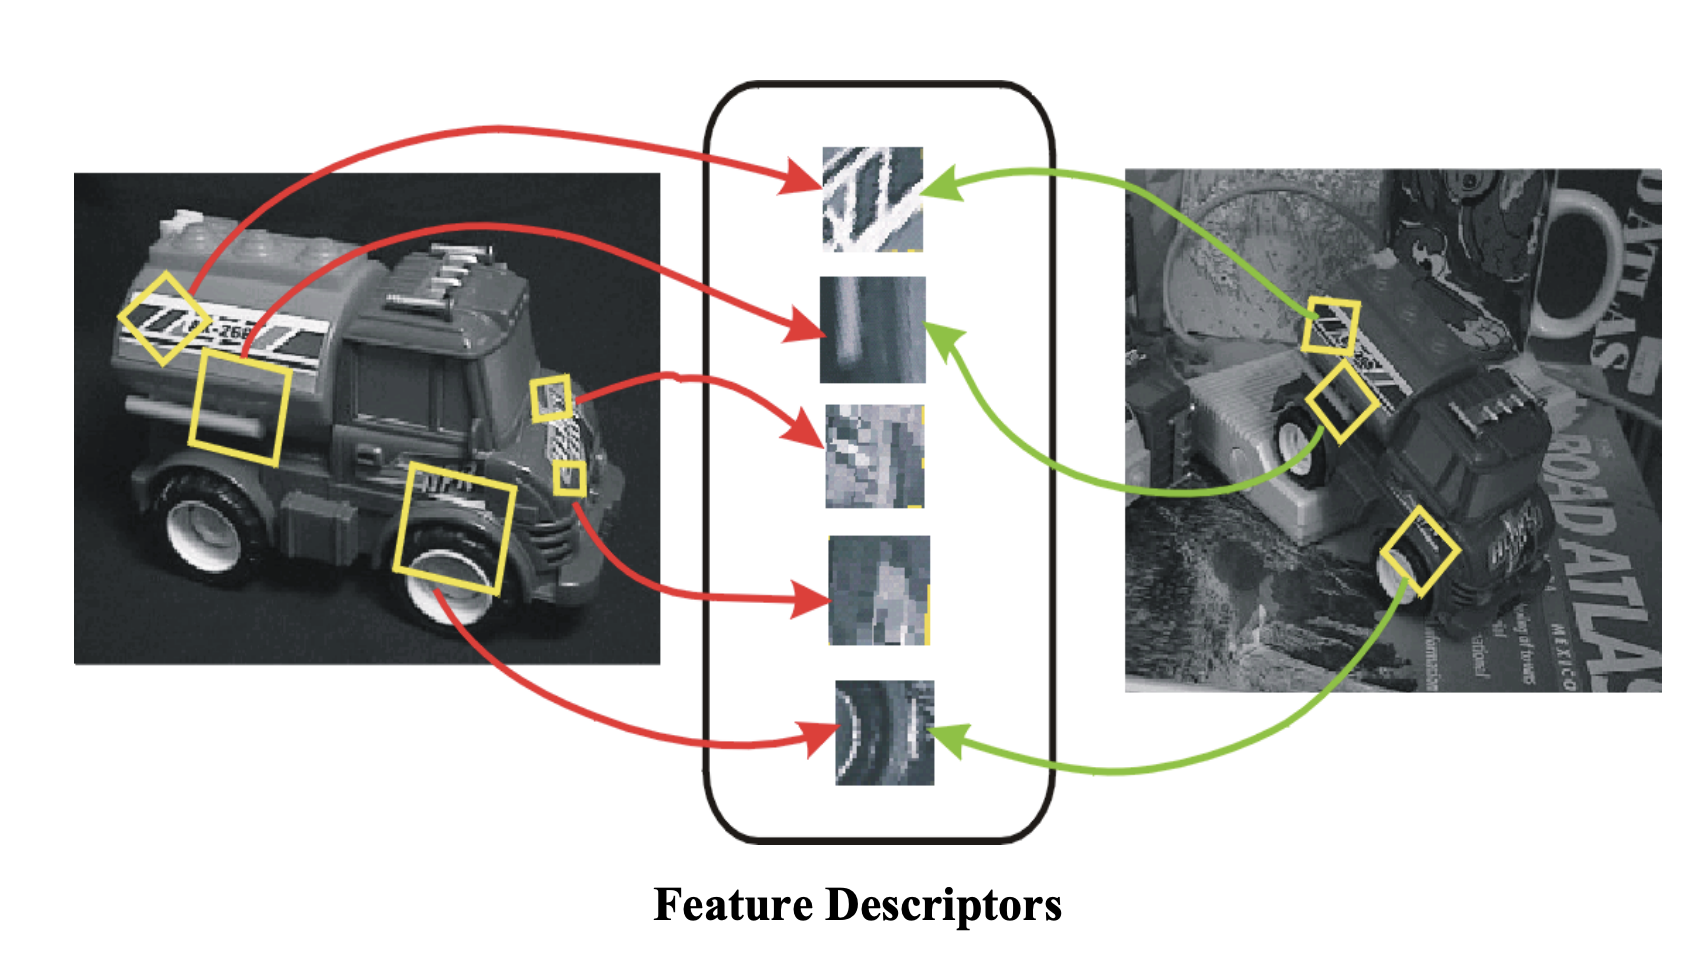
\includegraphics[width=0.7\textwidth]{img/invariantlocal.png}
    \caption{Patterns in images should remain the same even if picture changes}
\end{figure}
[Source: N. Snavely]
\end{frame}

\begin{frame}{Invariant Local Features}
    What are advantages of local features?
    \begin{itemize}
        \item Locality: features are local, so robust to occlusion and clutter
        \item Quantity: hundreds or thousands in a single image
        \item Distinctiveness: can differentiate a large database of objects
    \end{itemize}
\end{frame}

\begin{frame}{Invariant Local Features}
Suppose we only consider a small window of pixels
\begin{itemize}
    \item Look for image regions that are unusual: lead to unambiguous matches in other images
    \item How to define ”unusual”?
\end{itemize}
\end{frame}

\begin{frame}{Invariant Local Features}
Suppose we only consider a small window of pixels
\begin{itemize}
    \item What defines whether a feature is a good or bad candidate?
    \item (This intuition is used in the famous Harris Corner Detector)
\end{itemize}
 \begin{figure}
    \centering
    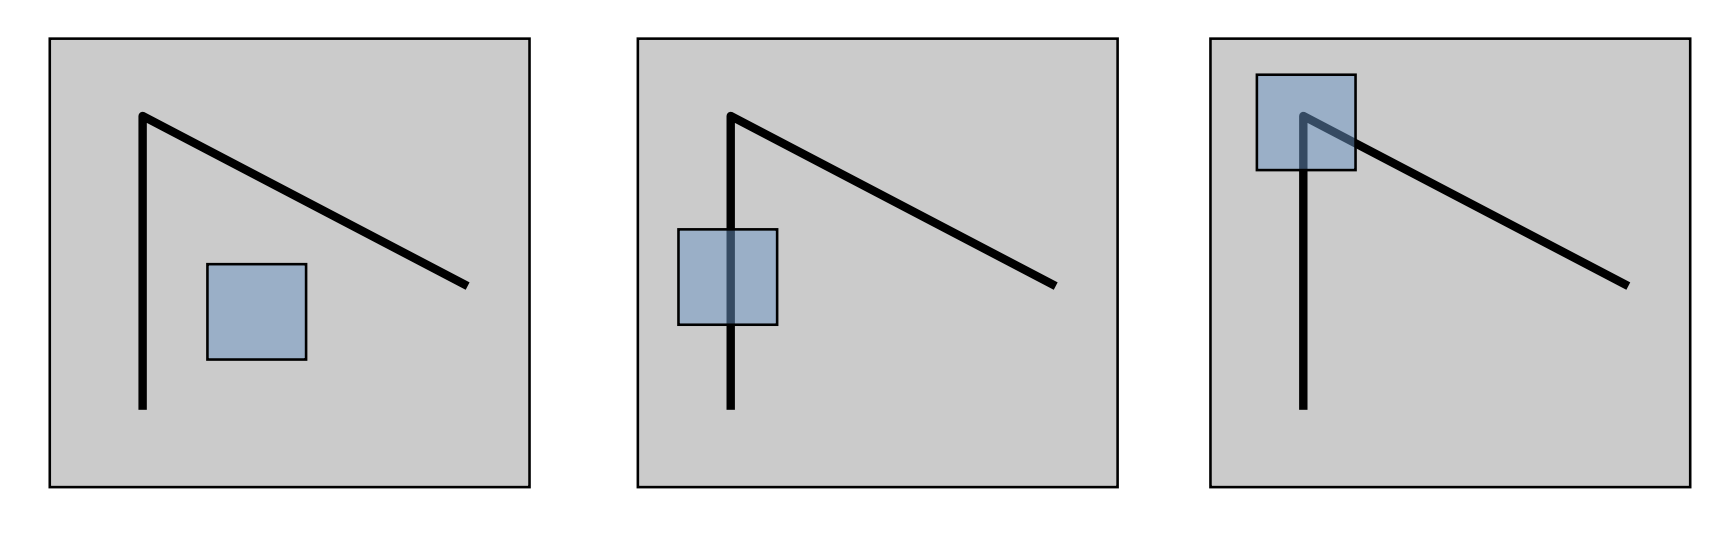
\includegraphics[width=0.7\textwidth]{img/edgebest.png}
    \caption{Which window would change the most if you shift it?}
\end{figure}  
    [Source: S. Seitz, D. Frolova, D. Simakov]

\end{frame}


